% interacttfssample.tex
% v1.05 - August 2017

\documentclass[]{interact}

\usepackage{epstopdf}% To incorporate .eps illustrations using PDFLaTeX, etc.
\usepackage[caption=false]{subfig}% Support for small, `sub' figures and tables
%\usepackage[nolists,tablesfirst]{endfloat}% To `separate' figures and tables from text if required

%\usepackage[doublespacing]{setspace}% To produce a `double spaced' document if required
%\setlength\parindent{24pt}% To increase paragraph indentation when line spacing is doubled
%\setlength\bibindent{2em}% To increase hanging indent in bibliography when line spacing is doubled

\usepackage[numbers,sort&compress]{natbib}% Citation support using natbib.sty
\bibpunct[, ]{[}{]}{,}{n}{,}{,}% Citation support using natbib.sty
\renewcommand\bibfont{\fontsize{10}{12}\selectfont}% Bibliography support using natbib.sty

\theoremstyle{plain}% Theorem-like structures provided by amsthm.sty
\newtheorem{theorem}{Theorem}[section]
\newtheorem{lemma}[theorem]{Lemma}
\newtheorem{corollary}[theorem]{Corollary}
\newtheorem{proposition}[theorem]{Proposition}

\theoremstyle{definition}
\newtheorem{definition}[theorem]{Definition}
\newtheorem{example}[theorem]{Example}

\theoremstyle{remark}
\newtheorem{remark}{Remark}
\newtheorem{notation}{Notation}

% Own definitions (Zoltan)
\usepackage{listingsutf8,newtxtt,xcolor,graphicx,xurl}
\lstset{language=Python,
  numbers=left,
  basicstyle=\ttfamily,
  keywordstyle=\bfseries\color{magenta},
  stringstyle=\color{red},
  numberstyle=\color{blue},
  breaklines=true,
  showstringspaces=false,
  backgroundcolor=\color{yellow!30},
  ndkeywordstyle=\color{magenta!70},
  commentstyle=\color{green},
  identifierstyle=\color{black},
  literate=
  {á}{{\'a}}1 {é}{{\'e}}1 {í}{{\'i}}1 {ó}{{\'o}}1 {ú}{{\'u}}1
  {Á}{{\'A}}1 {É}{{\'E}}1 {Í}{{\'I}}1 {Ó}{{\'O}}1 {Ú}{{\'U}}1
  {à}{{\`a}}1 {è}{{\`e}}1 {ì}{{\`i}}1 {ò}{{\`o}}1 {ù}{{\`u}}1
  {À}{{\`A}}1 {È}{{\'E}}1 {Ì}{{\`I}}1 {Ò}{{\`O}}1 {Ù}{{\`U}}1
  {ä}{{\"a}}1 {ë}{{\"e}}1 {ï}{{\"i}}1 {ö}{{\"o}}1 {ü}{{\"u}}1
  {Ä}{{\"A}}1 {Ë}{{\"E}}1 {Ï}{{\"I}}1 {Ö}{{\"O}}1 {Ü}{{\"U}}1
  {â}{{\^a}}1 {ê}{{\^e}}1 {î}{{\^i}}1 {ô}{{\^o}}1 {û}{{\^u}}1
  {Â}{{\^A}}1 {Ê}{{\^E}}1 {Î}{{\^I}}1 {Ô}{{\^O}}1 {Û}{{\^U}}1
  {Ã}{{\~A}}1 {ã}{{\~a}}1 {Õ}{{\~O}}1 {õ}{{\~o}}1
  {œ}{{\oe}}1 {Œ}{{\OE}}1 {æ}{{\ae}}1 {Æ}{{\AE}}1 {ß}{{\ss}}1
  {ű}{{\H{u}}}1 {Ű}{{\H{U}}}1 {ő}{{\H{o}}}1 {Ő}{{\H{O}}}1
  {ç}{{\c c}}1 {Ç}{{\c C}}1 {ø}{{\o}}1 {å}{{\r a}}1 {Å}{{\r A}}1
  {€}{{\euro}}1 {£}{{\pounds}}1 {«}{{\guillemotleft}}1
  {»}{{\guillemotright}}1 {ñ}{{\~n}}1 {Ñ}{{\~N}}1 {¿}{{?`}}1
  {Ω}{{$\Omega$}}1
  {ω}{{$\omega$}}1
  {→}{{$\to$}}1
  {ℝ}{{$\mathbb{R}$}}1,
  columns=fullflexible,
  keepspaces=true
}
\makeatletter
\def\lst@outputspace{{\ifx\lst@bkgcolor\empty\color{white}\else\lst@bkgcolor\fi\lst@visiblespace}}
\makeatother



\begin{document}

\articletype{ARTICLE TEMPLATE}% Specify the article type or omit as appropriate

\title{Towards understanding the central limit theorem by learning Python basics}

\author{
\name{Zolt\'an Kov\'acs\textsuperscript{a}\thanks{CONTACT Z. Kov\'acs. Email: zoltan@geogebra.org}
and Alexander Thaller\textsuperscript{b}}
\affil{\textsuperscript{a}
The Private University College of Education of the Diocese of Linz,
Salesianumweg 3, Linz, Austria;
\textsuperscript{b}Linz School of Education,
Altenberger Stra\ss e 54, Linz, Austria}
}

\maketitle

\begin{abstract}

We report on a first experiment about an email based course that connects learning
Python basics and introductory probability theory. In the experiment 7 short sequences
of homework were sent out to prospective mathematics teachers who did not have
any programming background formerly, but already had some minor knowledge on probability theory.
The experiment was about to decide if learning basics of programming can promote
understanding main concepts of probability theory.
\end{abstract}

\begin{keywords}
Python; programming; probability theory; central limit theorem
\end{keywords}

\section{Introduction}

We, the authors, have been spending a reasonable time with private tutoring in many fields
of mathematics---we are teachers. And, we agree on that probability theory is maybe
the most difficult field of mathematics---if it is about \textit{understanding}. For us, rough explanation
of statistical relationships seems to be easier than explaining the delicate issues
of properties of binomial coefficients, infinite sums and convergence. Indeed, in some
sense, statistics is much easier to explain---one needs to run virtual experiments
in a web browser % add links to Steve Phelps' https://www.geogebra.org/m/bxytp4hq, Ice Cream
% https://www.geogebra.org/m/qsjbqjfe, Broken Stick
% https://www.geogebra.org/m/bu5sxbn2, Fair Coin
% + Andreas Lindner's collections: https://www.geogebra.org/m/AytaSakt, https://www.geogebra.org/m/qXPnyCTZ
and this is well supported for several years, among others, in the online version of GeoGebra.

Connecting pure mathematics and real life or virtual experiments, can be, to our experience,
extremely hard. Probability is an important item of the curriculum at secondary level,
thus it is also an important item in the teacher training. But, to our experience,
most prospective teachers \textit{never} understand the basics beyond introductory level.
Our conjecture is that the main problem lies in students' verification if theory indeed meets practice,
so, at the end of the day, a very uncertain knowledge can be observed in the students' perception. As a consequence,
in most cases, not just yesterday's and today's mathematics teachers cannot connect
theory and practice, but their students either. Roughly speaking: everybody talks about probability and
statistics, but nobody understands anything behind the scenes.

In our paper we propose a radical way, or at least, to extend the classic way how
basics of elementary probability theory should be taught. It is \textit{programming}.
Our conjecture is that understanding will be significantly improved if the main concepts
of probability theory are supported with simple computer programs. The ouput for their flexible input
should be immediately checked, eventually in a web browser, and by changing the input parameters
to a higher number, the results can be quickly generalized. We emphasize that computers
can take on the high number of computatations from human---and this is what we exactly want.
A quite simple \textit{sample space} can contain \textit{a lot} of elements, even millions or more, and it cannot
be expected that non-experts can count their elements without deeper knowledge. In fact,
experts in probability are usually experts in combinatorics as well. To reach a reasonable
level of understanding of the main concepts in probability, by using just paper and pencil,
one needs to have a very strong and \textit{safe} background in combinatorics.

In this paper we demonstrate our proposal by explaining an email based course, sent out
to 4 prospective mathematics teachers, allowing them an arbitrary time to solve the problems being set.
The students claimed that they did not have any deeper knowledge in programming formerly, but all of
them already studied probability theory at university level. Their knowledge, however, was
not yet checked via examination. The course consisted of 7 sheets of homework assignments
and took place between November 2020 and January 2021, at the Johannes Kepler University of Linz, Austria.

\section{Preparations}
\label{preps}

First author hold a series of supplementary lectures on probability theory two years ago, where second author
took part a student and illustrated several homework assignments by using Python programs.
Some of his illustrations were a bit complicated for beginners, so the idea came that
simplified versions of such programs could be helpful for many students.
But, instead of giving a problem in probability theory and asking for a solution, in this
project we reversed the logic: We revealed the Python code in advance, and wanted to know
what problem will be solved with its help.

%\begin{figure}
%\lstinputlisting[language=Python]{../progs/de_AT/1.py}
%\caption{The first program in its original form (in German)}
%\label{1.py}
%\end{figure}

The first example is shown in Fig.~\ref{main-py-window}. We kept the original version to highlight
the possibility to write special characters in the Python code (we used Python version 3),
including accented German letters. In the first sheet of problems each student had to try
the code on his or her own on the website \url{https://repl.it/languages/python3},
by paying attention on the correct indentation as well---the students, however, did not have
to type the code but just copy it from the email into the programming window.
We also instructed all students with an
explanatory screenshot how the program should be started and the output obtained.

\begin{figure}
\begin{center}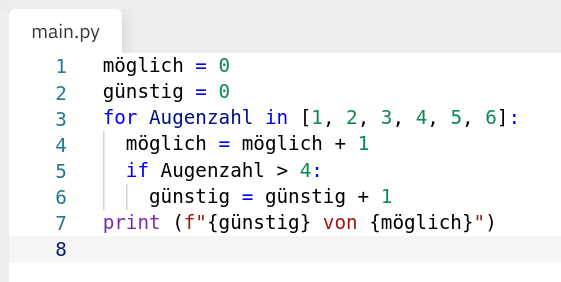
\includegraphics[scale=0.5]{../forms/de_AT/main-py-window}
\caption{An explanatory screenshot to help the students' first steps}
\label{main-py-window}
\end{center}
\end{figure}

In this introductory sheet the first question was to make the program work by running it,
and then explain its meaning line by line.
To give a somewhat creative assignment we also asked how the output $2/6$ can be changed to
the $3/6$. The outcome of this puzzle will be analyzed later in Section \ref{problem-sheets}.

It was expected that the students solve the sheet problems on their own, without
any communication. However, external help like using Internet was allowed for them.
The students were informed that about 6--8 sheets should be solved in the project,
and the required time for each should not exceed one hour.

In fact, we created a couple of other programs in advance, but always waited for
all solutions turned in by the students before finalizing the next sheet of problems.
We \textit{did not} give any feedback on their solutions. Instead, if we felt that
some difficulties arose, then we tried to cover them in the next sheet of problems.
The reason behind this was to test if it is possible to create a set of problems
\textit{in advance} for a possible \textit{static} learning path. Even if our experiment
was not fully static, for a future project now we already have a static set of materials.

Here we emphasize that easy access to an online version of a Python interpreter
played a significant role in our project. We did not want to ask the students
to install anything on their computer. Instead, we tried to minimize the gap
between theory and practice. In fact, \url{repl.it} is not the only website
allowing the user to try his or her code freely---we were just
satisfied with its simple user interface. Later, to obtain graphical output in an easy way, we also
introduced how Sage worksheets at \url{cocalc.com} can be accessed---in this latter case,
however, accented letters did not look elegant.

Importantly, we simplified and minimized the code we used during the email course.
This pre-process required several discussions among the authors to avoid
the technical difficulties of the programming language, but still allow
obtaining simple outputs. We had to balance between readability, simplicity,
elegance and speed. We learned that Python itself could be improved to
have simpler constructions than the \texttt{for i in range(...)} loop for iteration.
At the end of day we were still satisfied with all of the code and the students'
solutions confirm that our choices were acceptable.

As an example of a successful balance, we mention that we heavily used Python's support
for Unicode variable names.
We denoted the sample space by $\Omega$ and a single outcome by $\omega$ since
these notations were already well-known for the students. On the other hand,
typing these Greek characters is not straightforward: one may need to copy-paste
them since they are not available on a German keyboard.

\section{The problem sheets}
\label{problem-sheets}

\subsection*{Sheet 1}
The first sheet has already been mentioned in Section \ref{preps}.
The expected explanation of the Python program was solved well by the students.
All of them managed to write a correct answer to the creative question, namely
\begin{lstlisting}[language=Python,firstnumber=5]
  if Augenzahl > 3:
\end{lstlisting}
One student mentioned that the same output can be obtained with this change:
\begin{lstlisting}[language=Python,firstnumber=2]
günstig = 1
\end{lstlisting}
when line 5 is kept in its original form. Of course, this answer makes sense
only from the programmer's point of view, and it has less to do with probability.

After receiving the results for the first sheet we had the impression that
the students got familiar with the basics of the required technology.

\subsection*{Sheet 2}

The second sheet consisted of the following four questions:

\begin{enumerate}
\item Consider the following program:
\lstinputlisting[language=Python]{../progs/en_US/2.py}

\item Explain its meaning line by line, in one sentence for each.

\item Give the probability space where the possible outcomes are counted.
Which event has been identified here as ``desired''?

\item Modify the program to get a mechanical solution for the following question:

\begin{quote}
One fair die is rolled three times. Compute the probability for the event that the outcomes
correspond to a monotone increasing sequence.
\end{quote}

\end{enumerate}

We asked the students to try to solve the sheet problems without using any external help.
In case of lack of success
they were allowed to use a website that explains how to use if-then-else conditions in Python.

All students faced the quoted question during the introductory course in probability, but that time the solution
was expected to follow a purely pencil-and-paper method.

\subsubsection*{The results}

This sheet was much more difficult than the first one. One student reported that about an hour was required to solve it.
We learned that one student has a misconception by mixing relative frequency and probability---it was
a kind of surprise for this student that the program computes \textit{probability}, even if
there is no randomness built in. (In this case the students' misconception was corrected
by an explanation given in an email answer. Here we made an exception and forced
communication to clarify this basic concept.)

In general we were satisfied with the students' answers. All of them learned how three loops can
be nested to iterate on $\Omega=\{1,2,\ldots,6\}^3$. Multiple ways were found to express monotonicity,
including both the construct with an \texttt{and} clause and the short form
\texttt{outcome\_die\_1 <= outcome\_die\_2 <= outcome\_die\_3} which is one of Python's strengths.

In our experience it turned out that with little work a definitely large sample space
can be studied. In fact, manual check of $\{1,2,\ldots,6\}^3$ (or, equivalently, deriving the sum
$1+3+6+10+15+21$) is much more time consuming than writing a suitable program.

\subsection*{Sheet 3}

Fig.~\ref{3.py} shows the main code that was announced in the third sheet.

\begin{figure}
\lstinputlisting[language=Python]{../progs/en_US/3.py}
\caption{The third program (translated into English)}
\label{3.py}
\end{figure}

With this program we introduced some handy techniques via \texttt{itertools.product}
to define Cartesian powers. We pointed to
the second sheet and asked the students to rewrite their programs by using the new techniques.
We also asked them to display all desired outcomes on the screen (with the \texttt{print} command)
in a sorted fashion (via the \texttt{list} datatype).

We had positive feedback---they managed to understand the point. A student successfully generalized the 
solution for the puzzle of the second sheet for 5 dice, even if it was not directly asked.

\subsection*{Sheet 4}

The fourth sheet consisted of the following four questions:

\begin{enumerate}
\item Consider the following program:
\lstinputlisting[language=Python]{../progs/en_US/4.py}

\begin{enumerate}
\item Check if the program works properly. Save a screenshot for an evidence.
\item Explain the difference between this program and the one in sheet 3.
\end{enumerate}

\item Modify the program on line 7 and 14 in order to solve this problem:
\begin{quote}
Alice und Bob roll a die four times consecutively.
If the sum of the outcomes is between 7 and 14, Alice wins, otherwise Bob.
For which player is the game advantageous?
\end{quote}

\item Change the rules of the game above to get a fair play.
Verify the changed rules by writing a suitable program.

\item Assume that lines 12--15 are replaced by the following ones:
\begin{lstlisting}[language=Python,numbers=none]
E = [ω for ω in Ω if X(ω) == 10]
\end{lstlisting}
Check that the same result can be obtained as before.
Also, explain this short form by using a mathematical formula like a definition for a set.
\end{enumerate}

In this sheet we focused on the concept of random variables. To highlight their importance
we defined a Python function \texttt{X($\omega$)}.

\subsubsection*{The results}

The students answered the questions generally quite well. Two of them remarked that
the problem setting in question 2 was incomplete since line 10 has to be changed as well.

It turned out that the ``copy-paste'' way of copying a program was technically not always
straightforward---sometimes indentation was transferred improperly and some manual edit
was required on the student's side.

Fig.~\ref{42} shows a solution by a student for question 3. It is clear that this
student successfully combined previous programming knowledge, theory and praxis. Similarly,
two other students found the same idea to change the limits to have $7\leq X(\omega)\leq14$,
and one of them tried several attempts to find better limits---without success.
(Note that for an even number of dice there is no trivial solution by halving the
sample space symmetrically in the middle. So, in some sense, question 3 is adequate to motivate
experimenting.)

\begin{figure}
\begin{center}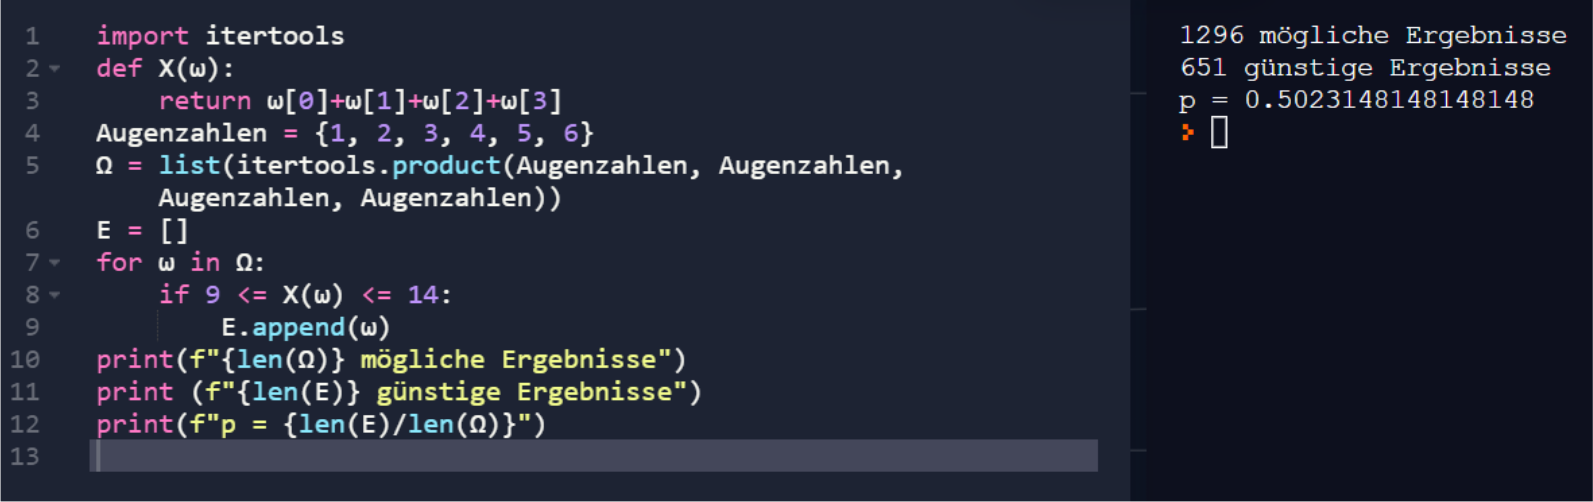
\includegraphics[width=1.0\textwidth]{42}
\caption{A student's solution for question 3 in sheet 4}
\label{42}
\end{center}
\end{figure}

The last question was solved perfectly by 3 students, giving the answer
$$E=\{\omega\;\mid\;\omega\in\Omega \land X(\omega)=10\}$$
where $X(\omega)=\omega_1+\omega_2$. Here we concluded that the technical
fact that Python's indexing starts from $0$, can be confusing for beginners,
since in mathematics the usual indexing starts from $1$.

\section*{Acknowledgement(s)}

\begin{thebibliography}{99}


\end{thebibliography}

\end{document}
